%                                                                 aa.dem
% AA vers. 7.0, LaTeX class for Astronomy & Astrophysics
% demonstration file
%                                                 (c) Springer-Verlag HD
%                                                revised by EDP Sciences
%-----------------------------------------------------------------------
%
%\documentclass[referee]{aa} % for a referee version
%\documentclass[onecolumn]{aa} % for a paper on 1 column  
%\documentclass[longauth]{aa} % for the long lists of affiliations 
%\documentclass[rnote]{aa} % for the research notes
%\documentclass[letter]{aa} % for the letters 
%
\documentclass[structabstract]{aa}  
%\documentclass[traditabstract]{aa} % for the abstract without structuration 
                                   % (traditional abstract) 
%
\usepackage{graphicx}
%%%%%%%%%%%%%%%%%%%%%%%%%%%%%%%%%%%%%%%%
\usepackage{txfonts}
%%%%%%%%%%%%%%%%%%%%%%%%%%%%%%%%%%%%%%%%
%
\usepackage{epsfig}
\usepackage{natbib}
\usepackage{lscape}
\usepackage{wasysym}
\usepackage{array}
\usepackage{amssymb}
\usepackage{subfigure}
%\usepackage{multicol}
\usepackage{longtable}
\usepackage{rotating}
\usepackage{color}
\usepackage{colortbl}
\usepackage{soul}
\usepackage[normalem]{ulem}
\usepackage{fancyheadings}
\bibpunct{(}{)}{;}{a}{}{,}

\newcommand\T{\rule{0pt}{2.6ex}}
\newcommand\B{\rule[-1.2ex]{0pt}{0pt}}

\begin{document}
%
   \title{Metallicity of M dwarfs}

   \subtitle{III. Planet-metallicity relationship on the HARPS GTO M dwarf sample}

\author{ V. Neves\inst{1,2,3} \and X. Bonfils\inst{2} \and
  N. C. Santos\inst{1,3} \and X. Delfosse\inst{2} \and
  T. Forveille\inst{2}  \and F. Allard\inst{4}  \and
  S. Udry\inst{7}}

\institute{
Centro de Astrof{\'\i}sica, Universidade do Porto, Rua das Estrelas,
4150-762 Porto, Portugal \\
email: {\tt vasco.neves@astro.ua.pt}
\and
UJF-Grenoble 1 / CNRS-INSU, Institut de Plan\' etologie et
d'Astrophysique de Grenoble (IPAG) UMR 5274, Grenoble, F-38041,
France.
\and
Departamento de F\'{\i}sica e Astronomia, 
Faculdade de Ci\^{e}ncias, Universidade do Porto, 
Rua do Campo Alegre, 4169-007 Porto, Portugal
\and
Centre de Recherche Astrophysique de Lyon, UMR 5574: CNRS,
Universit\'e de Lyon, \'Ecole Normale Sup\'erieure de Lyon, 46 All\'ee
d'Italie, F-69364 Lyon Cedex 07, France
}


   \date{Received XXX; accepted XXX}

% \abstract{}{}{}{}{} 
% 5 {} token are mandatory
 
  \abstract
  % context heading (optional)
  % {} leave it empty if necessary  
   {Here we study the relationship between metallicity and the frequency of planets and stars with planets}
  % aims heading (mandatory)
   {   }
  % methods heading (mandatory)
   {  }
  % results heading (mandatory)
   {   }
  % conclusions heading (optional), leave it empty if necessary 
   {}

   \keywords{no key words -- no no no
               }

   \maketitle
%
%________________________________________________________________

\section{Introduction}

%\textcolor{red}{Still don't know if I'm going to write a full introduction or just a resume of the previous paper and 3/4 paragraphs.}
\textcolor{red}{Should I disentangle theory from observations? - NOTE: Reduce the part talking about  the planet-metallicity correlation}

\textbf{The most basic observables used as input quantities in} core-accretion models of formation and evolution of planets around M dwarfs and other stars are mass and metallicity, as shown by numerous works studying the relationship of both quantities with planet formation \citep[e.g.][]{Ida-2005,Kornet-2006, Kennedy-2008a, Thommes-2008, Alibert-2011, Mordasini-2012}. \textcolor{red}{reformulate this paragraph }

The planets that orbit M dwarfs form in a different environment than solar-type and higher mass stars, as the initial conditions of formation (disk mass, temperature and density profiles, gravity, gas-dissipation and migration timescales...etc.) all change with stellar mass \citep[e.g.][]{Ida-2005, Kornet-2006, Kennedy-2008a, Alibert-2011}.  \textbf{Additionally}, metallicity also plays a major role in the efficiency of the formation of giant planets for FGK dwarfs, as shown by both models \citep[e.g.][]{Ida-2004b} and observational data \citep[e.g.][]{Gonzalez-1997,Santos-2004b,Fischer-2005, Mayor-2011}. Recently, it has been also shown that this trend might also be true for M dwarfs \citep[e.g.][]{Bonfils-2007,Johnson-2009, Schlaufman-2010, Rojas-Ayala-2012, Terrien-2012}. 

Moreover, the metallicity effect may be independent or only lightly dependent on the stellar mass effect \citep{Johnson-2010,Alibert-2011}. It remains to be seen, however, if the planet-metallicity correlation that seems to vanish for Neptunian and smaller planet hosts around FGK dwarfs \citep[][Guezzi-2010?]{Sousa-2008,Bouchy-2009,Sousa-2011b} and predicted by models \citep[e.g.][]{Mordasini-2012} is observed around M dwarfs \citep[e.g.][]{Rojas-Ayala-2012,Terrien-2012}.



%Ida 2005 and Kornet 2006 consider that giant formation around more massive stars than the sun is less likely, in contrast with KK2008a

% Kornet 2006 concludes that jupiter hosts are more common around less massive stars, that differs from Laughlin 2004 and Ida 2005.

% Mordassini 2009 a,b --> using only solar mass, b is more important. About PMC (feh).

% Mardasini 2012 --> feh effect is confirmed for giant planets. no feh effect for neptunians and for SE it might be an anti-correlation. No correlation between feh and distance for giant planets. low feh planets start further out, but migrate more, while at high feh they start closer in but migrate less! disk masses and giant planets are correlated. disk lifetime acts as a threshhold for giants formation. There is a compensation effect between mass and feh. feh effect is stronger when disk mass is weaker and vice versa.

% Laughlin 2004 - formation of giants around M dwarfs is inhibited.

%Ida 2004 - Gas giants and range of metallicities --> dependence of gas giant formation on feh

%Ida 2005 - lower mass planets may be more common around M dwarfs, because M dwarfs tend to migrate before starting gas accretion. The formation of Giant planets around M dwarfs is inhibited.

% Ida 2008b, Ida 2010 - frequency of SE around solar type stars

% discuss the question about disk lifetimes?

% Alibert 2010 --> study on mass with planet formation efficiency. The minimum metallicity required to form a massive planet is correspondingly lower for massive stars than lower mass stars.



According to \citet{Thommes-2008} and \citet{Mordasini-2012}, a lower metallicity can be compensated by higher disk masses to allow giant planet formation (and vice-versa -- the so called `compensation effect'). This result implies that M dwarfs can form giant planets, but only if they have high metallicities, thus suggesting a stronger planet-metallicity correlation on these stars compared to FGK dwarfs. 

Disk instability models \citep[e.g.][]{Boss-1997}, on the other hand, do not predict the dependence of the planet formation of stellar quantities such as stellar mass \citep[e.g.][]{Boss-2006a} and metallicity \citep{Boss-2002}. Contrary to the core-accretion paradigm \citep{Pollack-1996}, the formation of planets do not originate from the collisional accretion of planetesimals, but from the collapse of an unstable part of the protoplanetary disk, forming in a timescale of thousands of years when compared to a timescale of Myrs for core-accretion models. Observational evidence, however, has shown that there is indeed a dependence between planet occurrence and both stellar mass and metallicity \citep[e.g.][Johnson-2010]{}, thus favoring the core-accretion scenario as the primary mechanism of planet formation, at least for closer-in planets. 

In this context, the pollution scenario \citep[e.g.][]{Murray-2002}, defends that the observed enhanced metallicity is only at the surface of the photosphere, and that the formation of planets occurs at all metallicities, thus supporting disk instability models. Observationally, this would translate, for M dwarfs into a non-detection of the planet-metallicity correlation, as M dwarfs have very deep convective layers and are expected to be fully convective at masses below 0.4 M$_{\odot}$. However, as we've seen, most studies hint or demonstrate the presence of the correlation for giant planets, thus signaling a primordial origin of the presence of metals.

Observationally, the occurrence rate of hot jupiters around FGK stars is no bigger than 2\% \citep[e.g.][]{Howard-2010,Mayor-2011}. On M dwarfs this number may be even lower, showed by both works on models \citep[e.g.][]{Laughlin-2004,Ida-2005, Kennedy-2008a} and observations \citep[e.g.][]{Endl-2006, Cumming-2008,Johnson-2010,Bonfils-2011}. The paucity of hot jupiters around M dwarfs is most probably due to an inefficient planet-formation process around M dwarf protoplanetery disks (Laughlin-2004, Ida-2005, Kennedy-2008a). Whether or not this paucity of Gas giants around M dwarfs extends to higher periods and beyond the snow line remains to be seen. 

\citet{Gould-2010} estimates that the frequency of giant planets beyond the snow line around low mass stars can be as high as $0.36\pm15$. However, the upper limits and frequencies for different period regions from 1 to 10.000 days calculated by \citet{Bonfils-2011} taking into account the detection limits of radial velocity shows, in their Table 11, that the frequency beyond the snow line is only $0.04^{+0.05}_{-0.01}$ and is even lower for closer regions to the star. \textcolor{red}{This last part is open for discussion, of course. I don't understand the numbers of Gould-2010.}. Moreover, previous works \citep{Butler-2006,Cumming-2008} publish an even lower planet fraction for M dwarfs ($\sim$ 2\%) for periods below 2000 days. 



In this work, we derive the metallicities of a sample of 102 M dwarfs from the HARPS GTO programme. We implement a new method, using the high-resolution spectra of HARPS, described in the Appendix, to refine and enhance the precision of metallicities based on the photometric calibration of \citet{Neves-2012}, itself a refinement of the work of\citet{Schlaufman-2010}. Then, we use this determinations, as well as stellar mass determinations calculated using the mass-luminosity relation of \citet{Delfosse-2000} to search for correlation between the frequency of planets with stellar mass and metallicity. In Sect. \ref{sample}, we describe our M dwarf sample and observations using the HARPS spectrograph. Then, in Sect. \ref{relation}, we investigate the stellar mass/metallcity correlations with the frequency of planets. Afterwards, we calculate the detection limits of the sample, to check for biases in our sample, since the planet detections accumulate in the higher end of stellar mass and lower end of V magnitude. Finally, we discuss our results in Sect. \ref{discussion}.

\textcolor{red}{Add wright 2012 to the hot jupiter discussion}






%The fact that ho 



%Efficiency of giant planets should increase with stellar mass (Laughlin 2004, Ida 2005b Kennedy 2007)

%No clear metallicity effect is found in the Neptunian mass domain and at lower masses even an anti-correlation might exist. (Mordassini 2012)

%Disk gas masses and giant planet masses are correlated (Mordassini 2012). 

%BUT Microlensing surveys show that 

%Mdisk is proportional to the Mdisk^alphad



%Alibert 2011 states that the number of embryos that eventually evolve and form planets are a growing function of the stellar mass. 

%The minimum metallicity required to form a massive planet is correspondingly lower for massive stars than lower mass stars. 
%
%However, \citet{Alibert-2011} states that the metallicity efffect is only weakly dependent on stellar mass. 

%--> Talk about the paucity of jovians around M dwarfs

%--> Should we talk about Disk instability?









%__________________________________________________________________

\section{Sample and Observations}
\label{sample}

Our 102 M dwarf sample is described in Sec. 2 of \citet{Bonfils-2011}. It is a volume limited (11 pc) HARPS sample, containing stars with a declination $\delta< +20^{\circ}$, with V magnitudes brighter than 14  mag and including only stars with a projected rotational velocity $vsini\le 6.5$ km/s. All known spectroscopic binaries and visual pairs with separation lower than 5 $arcsec$, as well as previously unknown fast rotators were removed \textit{`a priori'} or \textit{`a posteriori'} from the original sample. 

From the 102 M dwarf stars, a total of 14 planets are currently detected, in 8 star systems, from which 3 have more than one planet. 

\textcolor{red}{should we put here the Table 1 of Bonfils(2011) but only including our sample? Should we put more information regarding the sample(observations?}

The stellar masses were calculated using the empirical mass-luminosity relationship of \citet{Delfosse-2000}, using stellar parallaxes (taken mostly from the HIPPARCOS catalogue \citep{van_Leeuwen-2007} , but also from \citet{van_Altena-1995, Jahreiss-1997, Hawley-1997, Henry-2006}), V band magnitudes (taken from the Sinbad database\footnote{http://simbad.u-strasbg.fr/simbad/}), and the infrared K$_{s}$ magnitudes from 2MASS \citep{Skrutskie-2006}. The stellar mass values range from 0.09 to 0.60 $M_{\odot}$, with a mean and median values of 0.32 and 0.29 $M_{\odot}$ respectively. We note that Gl 803, a young ($\sim 20$ Myr) M dwarf with a circumstellar disk \citep{Kalas-2004}, has a stellar mass value of 0.75, too high for a M dwarf. This means that the stellar mass calibration being used may not be adequate to measure young M dwarfs. 

The metallicities were first calculated with the photometric calibration provided by \citet{Neves-2012}, based on the work of \citet{Schlaufman-2010}, using stellar parallaxes, and V and K$_{s}$ magnitudes. \textcolor{red}{Neves or Schlaufman calibration? It's very hard to choose one, but the Schlaufman has a higher rms = 0.11, although it also has a wider range of metallicities. BUT we can compare it with the metallicity of 451GTO, and here the Schlaufman one clearly wins.} Then, a refinement of this calibration was done with the method described in the Appendix, using the measurements of the areas of the lines and features of the 26 red orders of the HARPS spectra. We achieve an increase in precision with the new calibration reaching a [Fe/H] dispersion of the order of 0.08 dex. The metallicity values range from -0.81 to 0.26 dex, with a mean and median values of -0.14 and -0.12 dex respectively. We note that there is an offset towards lower metallicities when compared with the 451 FGK dwarfs from the HARPS GTO sample \citep{Sousa-2008} with mean and median values of -0.09 and 0.08 dex respectively. \textcolor{red}{Using the calibration of SL10 we have a mean of -0.12 and a median of -0.10 dex. Is the use of the spectra pushing the metallicities towards lower values, due to the molecular lines??}.

\textcolor{red}{A table with masses and metallicities for the first 10 stars is needed in here, I think.}

The observations were gathered using the HARPS instrument (\citet{Mayor-2003b,Pepe-2004}, installed at the ESO 3.6-m telescope at the La Silla observatory in Chile. It is a high resolution (R$\sim$115000) spectrograph in the visible, covering a region between 3800 and 6800 \AA. During the time of the GTO program, from 11th February 2003 to the 1st of April 2009, a total of 1965 spectra were recorded. The aim of the HARPS M dwarf programme is to achieve a $\sim 1$ m/s RV precision per exposure for the brighter targets. The chosen recording mode during this period was single fiber mode, that relies only on a single calibration but gives enough precision to reach the aim of the programme. Using single fiber mode has the advantage of obtaining non-contaminated spectra that can be used to perform other studies such as calculating stellar parameters and abundances other than measuring the star's RV. A more detailed description of the observations is given in Sect. 3 of \citet{Bonfils-2011}.

\section{Stellar mass, metallicity, and planets}
\label{relation}

In this section we use the new metallicity values as well as the stellar mass determinations to study the possible correlations of these quantities with the planet frequency.

Figure \ref{histfull} shows the histograms of stellar mass (upper panel) and metallicity (lower panel) of our sample. The red histograms represent the stars without planets, while the blue histograms the stars with planets. The vertical solid and dashed lines above each histogram depict the value of the mean and the median respectively. %We note that there is a lower count in the 0.35-0.40 M$_{\odot}$ bin. We attribute this to statistical fluctuations due to the small number of each bin. \textcolor{red}{what else???}.


\begin{figure}[h]
\begin{center}
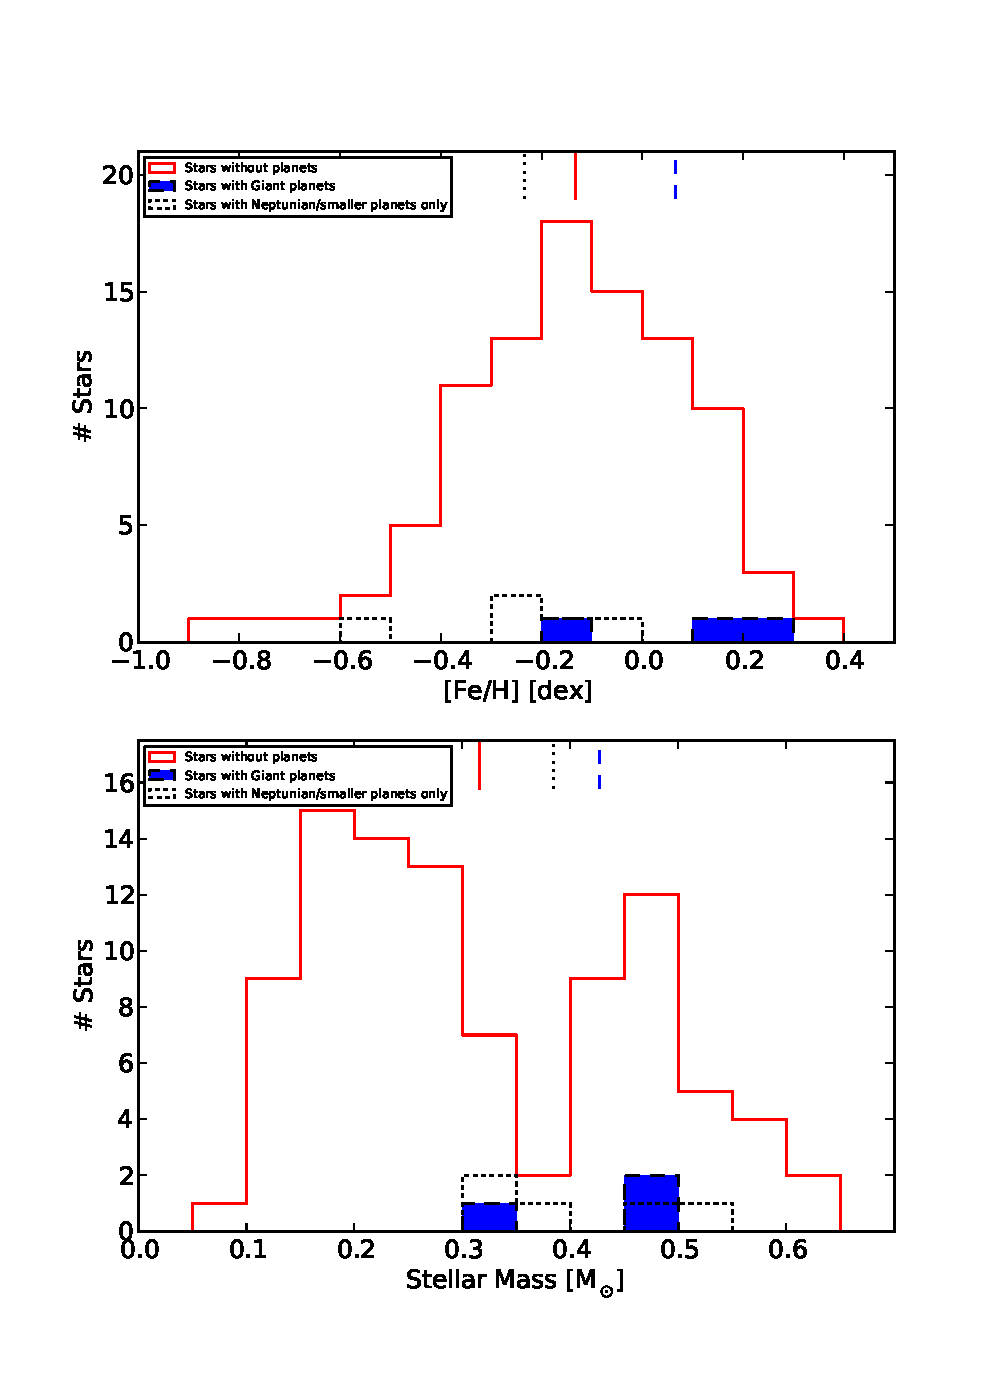
\includegraphics[scale=0.6]{../harpsm/all/pics_harpsmgtovpaper/histfull.eps}
\end{center}
\caption{Histograms of stars without planets (solid red) and with planets (dashed blue) for stellar mass (upper panel) and metallicity (lower panel). The vertical solid and dashed lines represent the mean and median of each distribution, respectively.}
\label{histfull}
\end{figure}


We can observe that, for stellar mass, there is a 0.08 $M_{\odot}$ (0.12 $M_{\odot}$ resp.) difference between the means (medians resp.) of planet and non-planet host histograms. Regarding metallicity, this difference is smaller (0.05 and 0.02 dex between the means and the medians, respectively). We performed a Kolmogorov-Smirnov (KS) test to the samples of stars with and without planets, for stellar mass and metallicity, and obtained p-values of 0.01 and 0.96 respectively. Therefore, regarding stellar mass, there is a low 1\% probability that the stars with and without planets are drawn from the same distribution, suggesting a real, if marginal, difference between the samples, in accordance with similar studies for M dwarfs \citep{Johnson-2007,Johnson-2010} as well as for AFGK dwarfs \citep{Laws-2003,Lovis-2007,Johnson-2010}. \textcolor{red}{check these references.........!!! and put some model references}. %\textcolor{red}{It is interesting to see that, if we divide the planet host sample into one subgroup having only Jupiter-type planets (N=3) and into another subgroup having Neptunian and smaller type planets (N=5) we obtain similar values for the difference between planet hosts and non-planet hosts (. This is a hint that 

Regarding metallicity, the KS test gives a very high probability that both samples belong to the same distribution, thus not agreeing with previous results for giant planets around M dwarfs \citep[e.g.][]{Bonfils-2007,Johnson-2009,Johnson-2010,Schlaufman-2010,Rojas-Ayala-2010,Rojas-Ayala-2012,Terrien-2012}. However, this result is coherent with the [Fe/H] results for Neptunian type FGK host stars where the planet-metallicity relation seems to vanish \citep[e.g.][]{Sousa-2008,Bouchy-2009,Sousa-2011b, Mayor-2011}, \textcolor{red}{(ver Sousa-2011a - metal poor sample)}. This result may simply reflect the fact that we only have three systems in our sample having Jupiter-type planets, the rest being Neptunian-type and smaller type planets. Moreover, we must note that we only have 8 stars with planets within our sample, which should make us cautious regarding the results of the K-S test. 

If we only take into account the three planet host stars with jupiter-type planets, the difference between the mean and the median of stars with and without planets will be higher (0.15 and 0.29 dex respectively). On the other hand, if we remove the 3 systems with Jupiters, we obtain a mean and median of -0.01 and -0.05 dex respectively. The last two results hint that there may be a different type of planet formation for giant and Neptunian/Super Earth-type planets \citep[e.g.][more?]{Mordasini-2012}. \textcolor{red}{histogram picture for the jovians and neptunians here?,}
%For the same reason we did not study the frequency of giant planets around M dwarfs, as we only have three Jupiters type planets in two systems. 

%Nevertheless, if we separate the planet-host sample into two subgroups, with  divided by the sum of the planetary masses,

In order to explore the star-planet relation further with our limited number of stars with planets, we reduced the number of bins of the histograms of mass and metallicity to three and performed a frequency analysis, as shown in Figures \ref{3binmass} and \ref{3binfeh}, respectively. The upper panels of both Figures are the same as in Fig. \ref{histfull}, but this time with only three bins. The lower panels depict the relative frequency of the stars with planets. The frequency is calculated using the binomial distribution following the procedure outlined in, e.g., \citet[][]{Burgasser-2003,McCarthy-2004, Endl-2006}, and \citet{Sozzetti-2009}. The upper errors, lower errors and upper limits correspond to the 68\% of the integrated area around the peak of the probability distribution function, that corresponds to the 1$\sigma$ gaussian limit. 

\begin{figure}[h]
\begin{center}
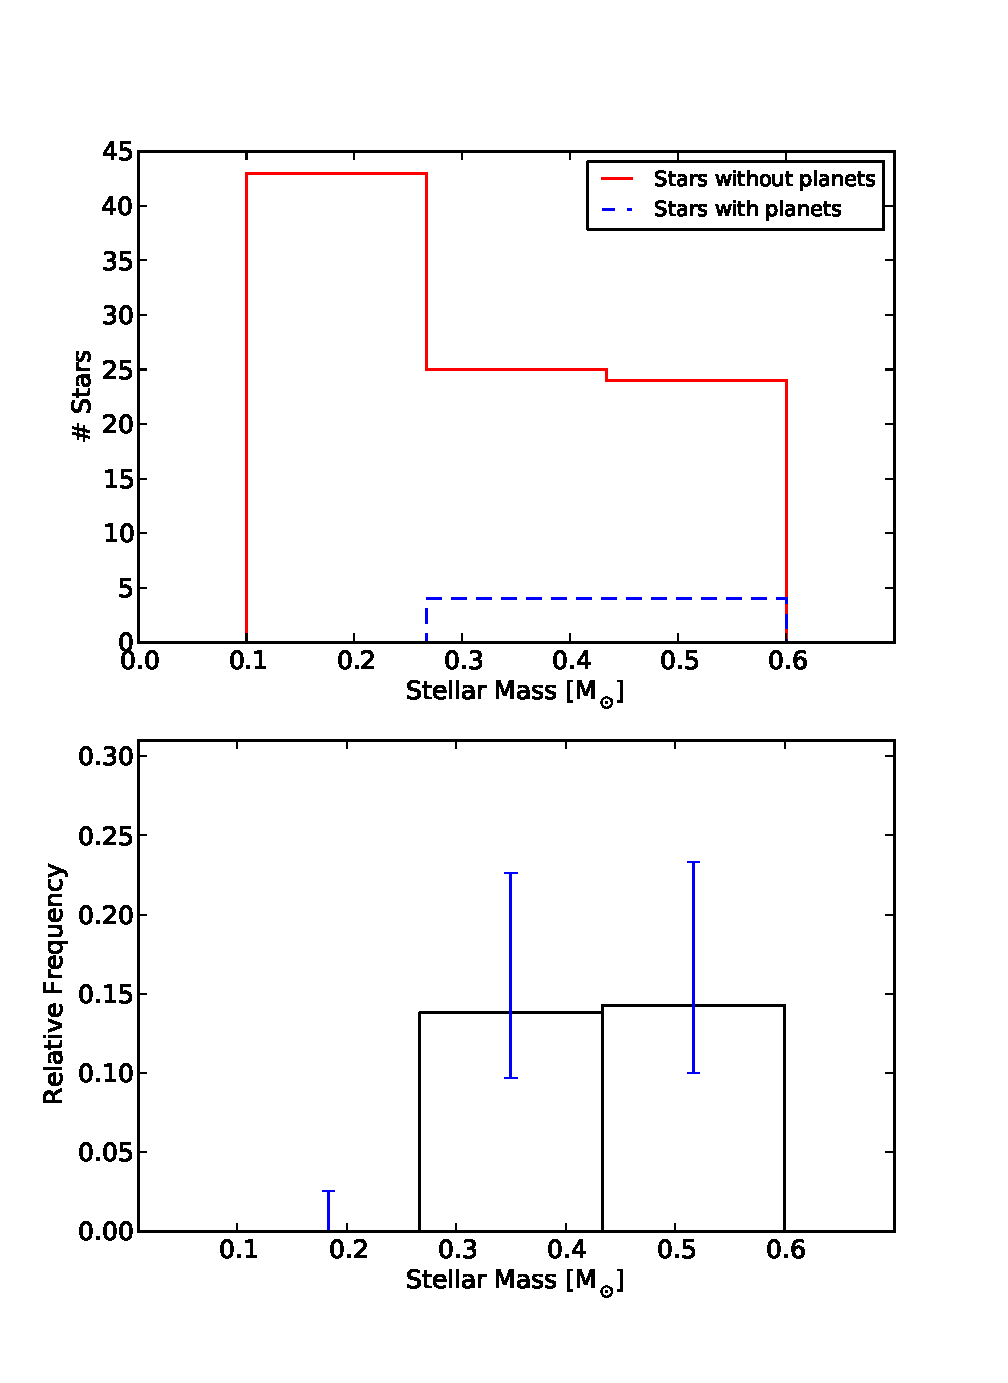
\includegraphics[scale=0.6]{../harpsm/all/pics_harpsmgtovpaper/3binmass.eps}
\end{center}
\caption{Upper panel: Histogram of stellar mass with 3 bins for stars without planets(solid red) and stars with planets (dashed blue); Lower panel: Frequency of stars with planets.}
\label{3binmass}
\end{figure}

\begin{figure}[h]
\begin{center}
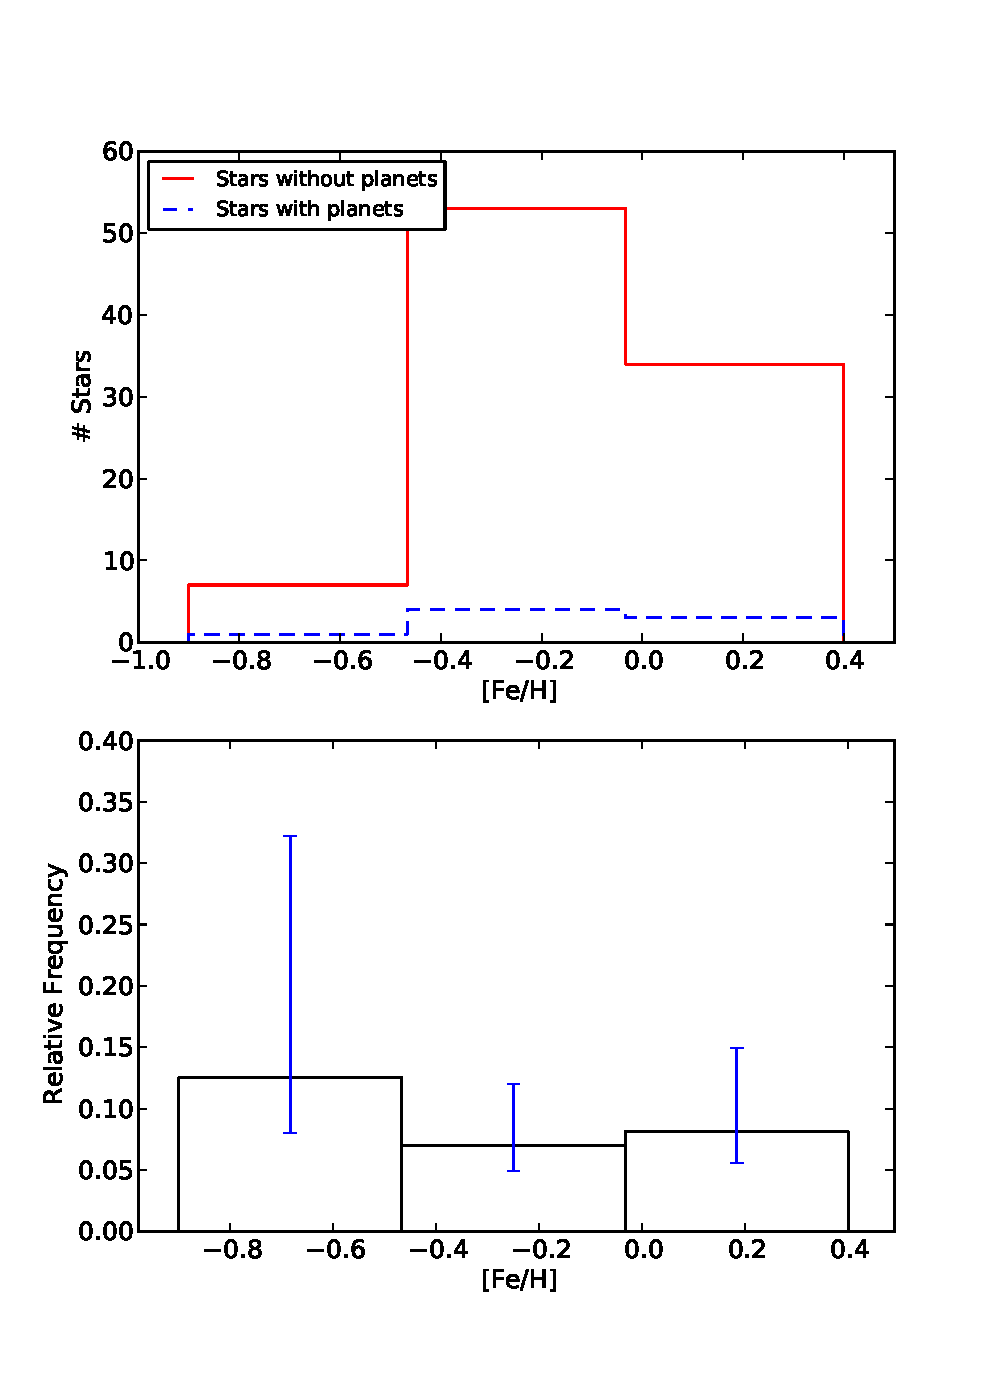
\includegraphics[scale=0.6]{../harpsm/all/pics_harpsmgtovpaper/3binfeh.eps}
\end{center}
\caption{Upper panel: Histogram of metallciity with 3 bins for stars without planets(solid red) and stars with planets (dashed blue); Lower panel: Frequency of stars with planets.}
\label{3binfeh}
\end{figure}

It can be seen that, for the frequency of planetary systems with stellar mass, there is a statistically significative difference ($> 3\sigma$)  between the upper limit of the first bin ( $0.1 < M_{\star} < 0.27$ and the values of the two higher stellar mass bins (up to 0.6 M$_{star}$). Quantitatively, the upper limit (1$\sigma$) of the first bin has a value of 0.0256 while the lowest value that the second bin can reach is 0.0966. This translates into a 3.7 $\sigma$ difference between the values of the two bins, meaning that we can already see a trend of planet frequency with stellar mass, even with only 8 stars with planets. However, we still have to check if this result is physical or due to a detection bias, as planets are easier to detect around more massive stars. In fact, the Fig. 1 of \citet{Bonfils-2011} (and Fig. \ref{histmass} of this work) shows that the planet detections are all on one side of the median of our sample distribution with V magnitude (all detected planets are around brighter stars) and stellar mass (all detected planets are around the more massive stars). This is will be adressed in Sect. \ref{dl}.

Regarding the frequency planet-host stars with metallicity, it can be clearly seen that there is no statistical difference between the bins. More detections are needed to test whether this non-correlation has a physical meaning or not. The simplest explanation for it is that it is only reflecting the higher number of lower mass being detect around M dwarfs, as, according to results obtained for FGK dwarfs, do not seem correlate with metallicity \citep[e.g.][]{Sousa-2011b}.



\section{Taking the detection limits into account}
\label{dl}

In order to check if there is any statistically significative bias due to the detection limits, we will first investigate the reason why all planet detections of our sample are located in the brightest and more massive halves of the two distributions, as can be seen in Fig. \ref{histmass}, for the stellar mass (similar to Fig. 1 of \citet{Bonfils-2011}). We attribute the low number of stars with a mass between 0.35 and 0.4 M$_{\odot}$ to a statistical fluctuation due to the small number of stars. \textcolor{red}{(I wonder why Fig 4. and Fig 1. of Bonfils 2011 are a bit different..... :O)}

\begin{figure}[h]
\begin{center}
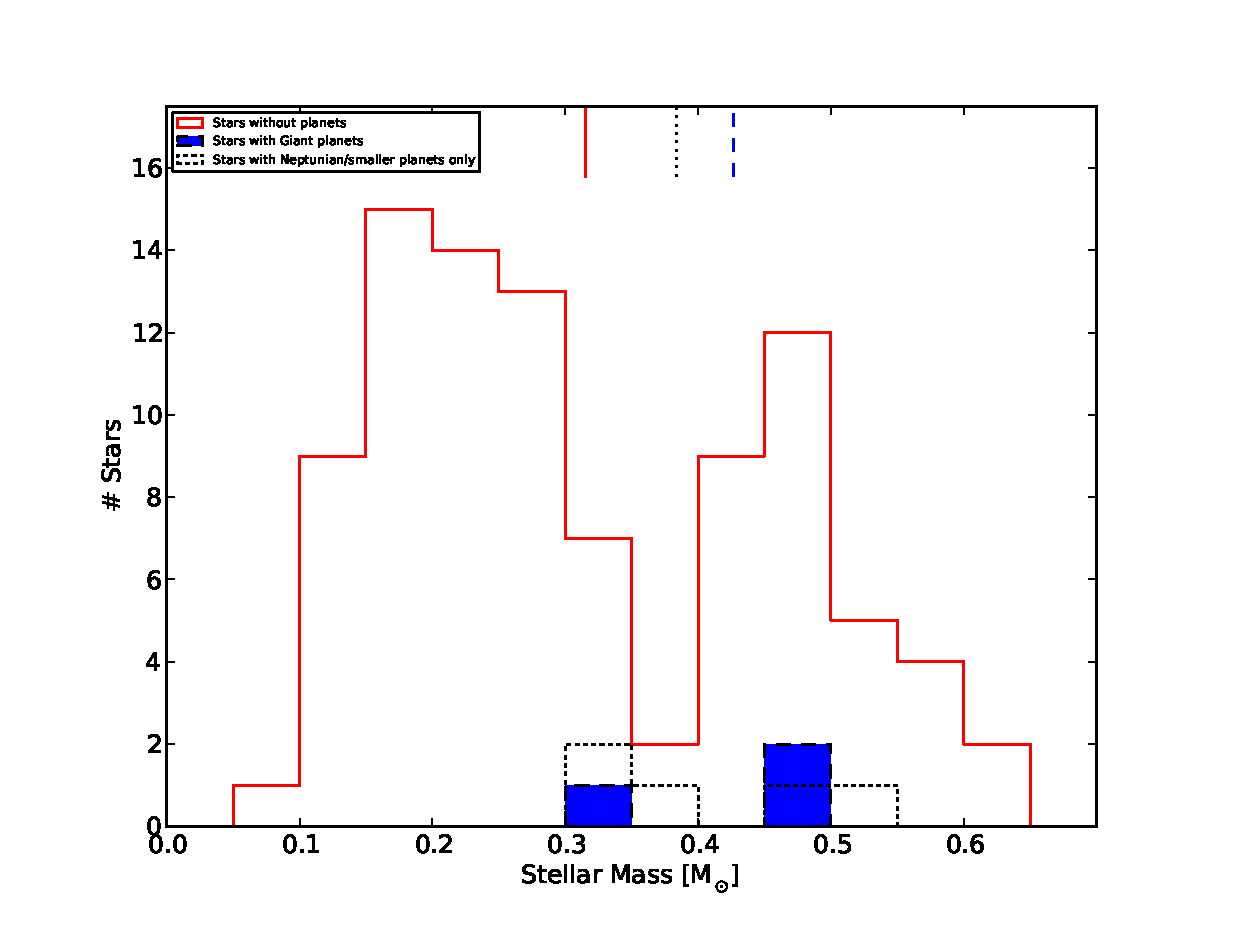
\includegraphics[scale=0.45]{../harpsm/all/pics_harpsmgtovpaper/histmass.eps}
\end{center}
\caption{Stellar mass distribution of the sample. The blue solid and dashed vertical lines represent the mean and the median of the stellar mass of the sample respectively. The black vertical lines locate the systems with planet detections.}
\label{histmass}
\end{figure}

In order to do this, we divide the sample into two stellar mass ranges by the median (0.29 M$_{\odot}$). We note that we removed the star Gl803 from the sample, due to the fact that the mass for this star may have not been adequately calculated, as explained in Sect. \ref{sample}. Then, we calculate the frequency of stars with planets, where multiplanetary systems are characterized by their most massive planet, and the frequency of planets. For both cases, we take into account the detection limits of our sample for different regions of the mass-period diagram following the procedure described in Sect. 7 of \citet{Bonfils-2011}. In short, for each region, we calculate the frequency $f=N_{d}/N_{\star,eff}$, where $N_{d}$ is the number of planet detections (or stars with planets) for each region, and $N_{\star,eff}$ is the number of stars whose detection limits exclude planets with similar mass and period at the 99\% confidence level. The N$_{\star,eff}$ is evaluated with Monte-Carlo sampling as described in \citet{Bonfils-2011}. The final $N_{\star,eff}$ value for each region is the average value of 10.000 trials. The confidence intervals are calculated in a similar fashion as described in Sect. \ref{relation} but this time using a poissonian distribution to calculate the 1$\sigma$ gaussian-equivalent area of the probability distribution.% limit equivalent confidence intervals.%, instead of using a binomial distribution. 

The results for the two halves of the stellar mass distribution can be seen in Table \ref{fswpl} and \ref{fswpu} for the frequency of stars with planets (N=8), and in Table \ref{fpl} and \ref{fpu} for the occurrence of planets (N=14). We observe that, in the stars with planets case, all values between the upper limits for M$_{\star} \le $0.29M$_{\odot}$ (Table \ref{fswpl}) and the values  for M$_{\star} > $0.29M$_{\odot}$ (Table \ref{fswpu}) are compatible with each other for all regions of planetary mass and period, except in the three regions with period between 10 and $10^{4}$ days, and mass between 1 and 10 M$_{\oplus}$, where we cannot compare the values due to a low N$_{eff}$ number. We observe the same regarding the results of the occurrence of planets (Tables \ref{fpl} and \ref{fpu}). 

\textcolor{red}{The fact that we do not observe a statistically significative ($> 2\sigma$) difference in any region of the mass-period diagram between the two stellar mass samples means that the difference between the frequencies of the first two bins in Fig. \ref{3binmass} is not detected, when we take into account the detection limits.This indicates that the observed difference is probably due to a stellar mass detection bias. We need more detections to check if a real stellar mass trend exists or not. DISCUSS!!!!what should be the strength of the argument here?}

%Other than that, we cannot conclude anything regarding whether the observed stellar mass-planet dependence in Fig \ref{3binmass} is true or if it is just an observational bias towards brighter/ more massive stars.

\begin{table}[]
\centering
\caption{Upper limits for the occurrence of stars with planets for M$_{\star} \leq 0.29$ $M_{\odot}$ (N$_{\star}$=52). }
\label{fswpl}
\begin{center}
\resizebox{9cm}{!}{
\begin{tabular}{l | c c c c}

\hline
\hline

                &  \multicolumn{4}{c}{Period} \\
$m\sin{i}$ & \multicolumn{4}{c}{[day]} \\

\multicolumn{1}{c |}{[M$_{\oplus}$]}  & $1-10$ & $10 - 10^{2}$ & $10^{2} - 10^{3}$ & $10^{3} - 10^{4}$ \\
\hline
$10^3 - 10^4$ & $N_{d}=0$ & $N_{d}=0$ & $N_{d}=0$ & $N_{d}=0$ \\
              & $N_{eff} = 47.51$ & $N_{eff} = 46.85$ & $N_{eff} = 45.74$ & $N_{eff} = 42.67$ \\
              & $f<0.02(1\sigma)$ & $f<0.02(1\sigma)$ & $f<0.02(1\sigma)$ & $f<0.03(1\sigma)$ \\
$10^2 - 10^3$ & $N_{d}=0$ & $N_{d}=0$ & $N_{d}=0$ & $N_{d}=0$ \\
              & $N_{eff} = 44.11$ & $N_{eff} = 41.19$ & $N_{eff} = 36.31$ & $N_{eff} = 24.39$ \\
              & $f<0.03(1\sigma)$ & $f<0.03(1\sigma)$ & $f<0.03(1\sigma)$ & $f<0.05(1\sigma)$ \\
$10 - 10^2$ & $N_{d}=0$ & $N_{d}=0$ & $N_{d}=0$ & $N_{d}=0$ \\
              & $N_{eff} = 28.56$ & $N_{eff} = 18.86$ & $N_{eff} = 9.90$ & $N_{eff} = 3.43$ \\
              & $f<0.04(1\sigma)$ & $f<0.06(1\sigma)$ & $f<0.12(1\sigma)$ & $f<0.31(1\sigma)$ \\
$1 - 10$ & $N_{d}=0$ & $N_{d}=0$ & $N_{d}=0$ & $N_{d}=0$ \\
              & $N_{eff} = 3.90$ & $N_{eff} = 1.45$ & $N_{eff} = 0.46$ & $N_{eff} = 0.01$ \\
              & $f<0.28(1\sigma)$ & $ - $ & $ - $ & $ - $ \\ [1pt]

\hline
\hline
\end{tabular}
}
\end{center}
\end{table}

\begin{table}[]
\centering
\caption{Frequencies and upper limits for the occurrence of stars with planets for M$_{\star} > 0.29$ $M_{\odot}$ (N$_{\star}$=49). Multiplanetary systems are characterized by their most massive planet.}
\label{fswpu}
\begin{center}
\resizebox{9cm}{!}{
\begin{tabular}{l | c c c c}

\hline
\hline

                &  \multicolumn{4}{c}{Period} \\
$m\sin{i}$ & \multicolumn{4}{c}{[day]} \\

\multicolumn{1}{c |}{[M$_{\oplus}$]}  & $1-10$ & $10 - 10^{2}$ & $10^{2} - 10^{3}$ & $10^{3} - 10^{4}$ \\
\hline
$10^3 - 10^4$ & $N_{d}=0$ & $N_{d}=0$ & $N_{d}=0$ & $N_{d}=0$ \\
              & $N_{eff} = 48.93$ & $N_{eff} = 48.73$ & $N_{eff} = 48.34$ & $N_{eff} = 47.24$ \\
              & $f<0.02(1\sigma)$ & $f<0.02(1\sigma)$ & $f<0.02(1\sigma)$ & $f<0.02(1\sigma)$ \\
$10^2 - 10^3$ & $N_{d}=0$ & $N_{d}=1$ & $N_{d}=0$ & $N_{d}=2$ \\
              & $N_{eff} = 47.79$ & $N_{eff} = 47.03$ & $N_{eff} = 44.74$ & $N_{eff} = 34.66$ \\
              & $f<0.02(1\sigma)$ & $f=0.02_{-0.01}^{+0.05}$ & $f<0.03(1\sigma)$ & $f=0.06_{-0.02}^{+0.08}$ \\
$10 - 10^2$ & $N_{d}=2$ & $N_{d}=0$ & $N_{d}=0$ & $N_{d}=0$ \\
              & $N_{eff} = 40.26$ & $N_{eff} = 31.78$ & $N_{eff} = 19.98$ & $N_{eff} = 7.18$ \\
              & $f=0.05_{-0.02}^{+0.07}$ & $f<0.04(1\sigma)$ & $f<0.06(1\sigma)$ & $f<0.16(1\sigma)$ \\
$1 - 10$ & $N_{d}=3$ & $N_{d}=0$ & $N_{d}=0$ & $N_{d}=0$ \\
              & $N_{eff} = 9.44$ & $N_{eff} = 3.89$ & $N_{eff} = 0.98$ & $N_{eff} = 0.10$ \\
              & $f=0.32_{-0.10}^{+0.31}$ & $f < 0.28 (1\sigma)$ & $ - $ & $ - $ \\ [1pt]
\hline
\hline
\end{tabular}
}
\end{center}
\end{table}

\begin{table}[]
\centering
\caption{Upper limits for the occurrence of planets for M$_{\star} \leq 0.29$ $M_{\odot}$ (N$_{\star}$=52).   }
\label{fpl}
\begin{center}
\resizebox{9cm}{!}{
\begin{tabular}{l | c c c c}

\hline
\hline

                &  \multicolumn{4}{c}{Period} \\
$m\sin{i}$ & \multicolumn{4}{c}{[day]} \\

\multicolumn{1}{c |}{[M$_{\oplus}$]}  & $1-10$ & $10 - 10^{2}$ & $10^{2} - 10^{3}$ & $10^{3} - 10^{4}$ \\
\hline
$10^3 - 10^4$ & $N_{d}=0$ & $N_{d}=0$ & $N_{d}=0$ & $N_{d}=0$ \\
              & $N_{eff} = 47.51$ & $N_{eff} = 46.85$ & $N_{eff} = 45.74$ & $N_{eff} = 42.70$ \\
              & $f<0.02(1\sigma)$ & $f<0.02(1\sigma)$ & $f<0.02(1\sigma)$ & $f<0.03(1\sigma)$ \\
$10^2 - 10^3$ & $N_{d}=0$ & $N_{d}=0$ & $N_{d}=0$ & $N_{d}=0$ \\
              & $N_{eff} = 44.13$ & $N_{eff} = 41.24$ & $N_{eff} = 36.45$ & $N_{eff} = 24.63$ \\
              & $f<0.03(1\sigma)$ & $f<0.03(1\sigma)$ & $f<0.03(1\sigma)$ & $f<0.05(1\sigma)$ \\
$10 - 10^2$ & $N_{d}=0$ & $N_{d}=0$ & $N_{d}=0$ & $N_{d}=0$ \\
              & $N_{eff} = 28.51$ & $N_{eff} = 18.84$ & $N_{eff} = 9.89$ & $N_{eff} = 3.46$ \\
              & $f<0.04(1\sigma)$ & $f<0.06(1\sigma)$ & $f<0.12(1\sigma)$ & $f<0.31(1\sigma)$ \\
$1 - 10$ & $N_{d}=0$ & $N_{d}=0$ & $N_{d}=0$ & $N_{d}=0$ \\
              & $N_{eff} = 3.92$ & $N_{eff} = 1.47$ & $N_{eff} = 0.47$ & $N_{eff} = 0.01$ \\
              & $f<0.28(1\sigma)$ & $ - $ & $ - $ & $ - $ \\ [1pt]
\hline
\hline
\end{tabular}
}
\end{center}
\end{table}

\begin{table}[]
\centering
\caption{Frequencies and upper limits for the occurrence of planets for M$_{\star} > 0.29$ $M_{\odot}$ (N$_{\star}$=49).    }
\label{fpu}
\begin{center}
\resizebox{9cm}{!}{
\begin{tabular}{l | c c c c}

\hline
\hline

                &  \multicolumn{4}{c}{Period} \\
$m\sin{i}$ & \multicolumn{4}{c}{[day]} \\

\multicolumn{1}{c |}{[M$_{\oplus}$]}  & $1-10$ & $10 - 10^{2}$ & $10^{2} - 10^{3}$ & $10^{3} - 10^{4}$ \\
\hline
$10^3 - 10^4$ & $N_{d}=0$ & $N_{d}=0$ & $N_{d}=0$ & $N_{d}=0$ \\
              & $N_{eff} = 48.92$ & $N_{eff} = 48.71$ & $N_{eff} = 48.34$ & $N_{eff} = 47.21$ \\
              & $f<0.02(1\sigma)$ & $f<0.02(1\sigma)$ & $f<0.02(1\sigma)$ & $f<0.02(1\sigma)$ \\
$10^2 - 10^3$ & $N_{d}=0$ & $N_{d}=2$ & $N_{d}=0$ & $N_{d}=2$ \\
              & $N_{eff} = 47.78$ & $N_{eff} = 47.02$ & $N_{eff} = 44.65$ & $N_{eff} = 34.48$ \\
              & $f<0.02(1\sigma)$ & $f=0.04_{-0.01}^{+0.06}$ & $f<0.03(1\sigma)$ & $f=0.06_{-0.02}^{+0.08}$ \\
$10 - 10^2$ & $N_{d}=2$ & $N_{d}=0$ & $N_{d}=0$ & $N_{d}=0$ \\
              & $N_{eff} = 40.23$ & $N_{eff} = 31.60$ & $N_{eff} = 19.75$ & $N_{eff} = 7.07$ \\
              & $f=0.05_{-0.02}^{+0.07}$ & $f<0.04(1\sigma)$ & $f<0.06(1\sigma)$ & $f<0.16(1\sigma)$ \\
$1 - 10$ & $N_{d}=5$ & $N_{d}=3$ & $N_{d}=0$ & $N_{d}=0$ \\
              & $N_{eff} = 9.46$ & $N_{eff} = 3.90$ & $N_{eff} = 0.99$ & $N_{eff} = 0.10$ \\
              & $f=0.53_{-0.15}^{+0.36}$ & $f=0.77_{-0.23}^{+0.75}$ & $ - $ & $ - $ \\ [1pt]

\hline
\hline
\end{tabular}
}
\end{center}
\end{table}
 

The results for the V magnitude distribution are essentially the same, so we will report only the stellar mass results. \textcolor{red}{do we need to explain why?}













\section{Discussion}
\label{discussion}

In this paper we investigate the stellar mass and metallicity correlation with planets. We use a new method, using the high-resolution spectra of HARPS, described in the Appendix, to refine and enhance the precision of the metallicities based on the photometric calibration of \citet{Neves-2012}, itself a refinement of the \citet{Schlaufman-2010} calibration.

Regarding stellar mass, we detect a significative difference between planet and non planet host stars. However, when we take the detection limits into account, we do not find any correlation. Therefore, we interpret the trend of stellar mass with planets as being due to a detection bias in our sample. Despite that, we need more detections to robustly confirm whether there is a true stellar mass trend or not.

We do not detect a trend of metallicity with the presence of planets. We attribute this non-correlation to the fact that we have only 3 planet-host stars with Jupiter-type planets. If we calculate the difference between the means and medians of planet-host and not planet-host distributions, for Jupiter-type hosts and Neptunian and smaller type hosts a significative difference emerges for Jupiter-type hosts. Quantitatively, we calculate this difference between the mean and the median as being 0.15 and 0.29 dex respectively. This result is in line with previous works \citep[e.g.][]{Bonfils-2007,Johnson-2009, Schlaufman-2010, Rojas-Ayala-2012, Terrien-2012}.Regarding the Neptunian and smaller planet hosts, the observed difference is negligible, agreeing with the results for Neptunian-type planets orbiting FGK-type dwarfs \citep[e.g][]{Sousa-2011b}. We must be cautious about the results, however, as we only have 8 planet hosts in our sample. Therefore we should consider this results as hints, that need more detections to be confirmed as true trends. 

%In this work, we derive the metallicities of a sample of 102 M dwarfs from the HARPS GTO programme. We use a new method, using the high-resolution spectra of HARPS, described in the Appendix, to refine and enhance the precision of metallicities based on the photometric calibration of \citet{Neves-2012}, itself a refinement of the \citet{Schlaufman-2010} calibration. Then, we use this determinations, as well as stellar mass determinations from \citet{Bonfils-2011}, calculated using the mass-luminosity relation of \citet{Delfosse-2000} to search for correlation between the frequency of planets and stellar mass and metallicity. In Sect. \ref{sample}, we describe the sample of M dwarfs and the observations using the HARPS spectrograph. Then, in Sect. \ref{relation}, we investigate the stellar mass/metallcity correlations with the frequency of planets. Afterwards, we calculate the detection limits of the sample, to check for biases in our sample, since the planet detections accumulate in the higher end of stellar mass and lower end of V magnitude. Finally, we discuss our results in Sect. \ref{discussion}.





\begin{acknowledgements}
We acknowledge the
support by the European Research Council/European Community under the
FP7 through Starting Grant agreement number 239953. NCS also
acknowledges the support from Funda\c{c}\~ao para a Ci\^encia e a
Tecnologia (FCT) through program Ci\^encia\,2007 funded by FCT/MCTES
(Portugal) and POPH/FSE (EC), and in the form of grant reference
PTDC/CTE-AST/098528/2008. VN would also like to acknowledge the
support from the FCT in the form of the fellowship SFRH/BD/60688/2009. 
\textcolor{red}{PUT sinbad and 2mass in the acknowledgements}      


\end{acknowledgements}

\bibliographystyle{aa}
\bibliography{mylib.bib}

\appendix

\label{appendix}

\section{A new M dwarf metallicity and temperature calibration based on line measurements of HARPS M dwarf spectra}

In this appendix we briefly explain the method that we used to estimate the metallicity of M dwarfs. First, we must note that this scale is not a direct spectroscopic calibration. Rather, it is an indirect method, based on the metallicity photometric calibration of \citet{Neves-2012} (being itself a slight refinement of the one of \citet{Schlaufman-2010}) and the effective temperature calibration of \citet{Casagrande-2008}. Therefore, we're solely improving the precision of the existing photometric calibration with the aid of measurements of lines and features of M dwarf spectra. 

\subsection{Calibration sample}

From the 102 M dwarf spectra of the \citet{Bonfils-2011} sample we initially chose 60 stars with S/N greater than 100. Six stars (Gl191, Gl285, Gl388, Gl699, Gl729, Gl803, GJ1125) were then discarded \textit{`a posteriori'}, either due to a bad correlation of the line measurements with either the reference metallicity or temperature scales, or due to a bad value of the radial velocity (GJ1125). We ended up with a sample of 54 stars in which we based our calibration. \textcolor{red}{see here why they were discarded in the first place -- Table of the stars here?}. 

\subsection{Method}
\textcolor{red}{In this subsection I am not sure if I should describe all the methods or to describe only the one we have chosen. I opted to give only the best one.}

From our calibration sample we first measured `peak to peak' line and feature areas using the 26 redder orders of median normalized HARPS spectra, ranging from 5340 to 6901 \AA. Here we consider features as blended lines. 

Then we calculate a linear fit of the line/feature measurements with the metallicity (taken from \citet{Neves-2012}) and effective temperature (taken from \citet{Casagrande-2008}), using a least squares approach. For each line/feature $i$ we have,

\begin{equation}
W_{i,m} = \alpha_{i}[Fe/H]_{m} + \beta_{i}T_{eff m} + \gamma_{i},
\end{equation}

where each $W_{i,m}$, $[Fe/H]_{m}$, and $T_{eff m}$ is a $m\times1$ vector,  $m$ being the number of stars in the calibration sample. The $\alpha$ and the $\beta$ are the coefficients related to metallicity and effective temperature, respectively, while $\gamma$ is an independent coefficient. 


Our aim here is to increase the metallicity precision using the photometric calibration as reference. In order to do this, we want to recover the values of the metallicity and temperature by doing a weighted least squares refit, taking into account the errors of the calculated coefficients of the first fit. 

The error of each coefficient is calculated as

\begin{equation}
\epsilon_{i} = \sqrt{RSS.J_{i,i}},
\end{equation}
where RSS is the residual sum of squares, expressed as
\begin{equation}
RSS = \frac{\sum{(x-x_{i})^{2}}}{n_{obs}-n_{coef}},
\end{equation}
and $J$ is the jacobian matrix. 

The total error of the coefficients can then be written as 

\begin{equation} 
\epsilon = \sqrt{\epsilon\alpha^{2}+\epsilon\beta^{2}+\epsilon\gamma^{2}}.
\end{equation}

Here we assume that both [Fe/H] and temperature are independent and do not correlate with each other. 

To calculate the weights for the least squares refit we just invert the squared errors of the coefficients, and normalize the expression,

\begin{equation}
E_{i} = \frac{1/\epsilon_{i}^{2}}{\sum{1/\epsilon_{i}^{2}}}.
\end{equation}

We then apply the weights using the $optimize.least squares$ routine in $python$. 

We also tried other methods, such as choosing groups of lines with a high correlation or partial correlation coefficients and then applying the same method as described in this subsection. However, the weighted least squares method using all 4441 lines performed best at minimizing both metallicity and effective temperature. 

\textcolor{red}{A plot of the best calibration here for Feh and teff?}

Using this method, we get a dispersion of metallicity and effective temperature of 0.08 dex and 70K respectively. We must note, however that this is a differential method, meaning that we get an improvement of the precision but the accuracy of the calibration, as well as systematic errors are tied to the original determinations of both [Fe/H] and temperature. 








\end{document}















%%%%%%%%%%%%%%%%%%%%%%%%%%%%%%%%%%%%%%%%%%%%%%%%%%%%%%%%%%%%%%
Examples for figures using graphicx
A guide "Using Imported Graphics in LaTeX2e"  (Keith Reckdahl)
is available on a lot of LaTeX public servers or ctan mirrors.
The file is : epslatex.pdf 
%%%%%%%%%%%%%%%%%%%%%%%%%%%%%%%%%%%%%%%%%%%%%%%%%%%%%%%%%%%%%%

%_____________________________________________________________
%                 A figure as large as the width of the column
%-------------------------------------------------------------
   \begin{figure}
   \centering
   \includegraphics[width=\textwidth]{empty.eps}
      \caption{Vibrational stability equation of state
               $S_{\mathrm{vib}}(\lg e, \lg \rho)$.
               $>0$ means vibrational stability.
              }
         \label{FigVibStab}
   \end{figure}
%
%_____________________________________________________________
%                                    One column rotated figure
%-------------------------------------------------------------
   \begin{figure}
   \centering
   \includegraphics[angle=-90,width=3cm]{empty.eps}
      \caption{Vibrational stability equation of state
               $S_{\mathrm{vib}}(\lg e, \lg \rho)$.
               $>0$ means vibrational stability.
              }
         \label{FigVibStab}
   \end{figure}
%
%_____________________________________________________________
%                        Figure with caption on the right side 
%-------------------------------------------------------------
   \begin{figure}
   \centering
   \includegraphics[width=3cm]{empty.eps}
      \caption{Vibrational stability equation of state
               $S_{\mathrm{vib}}(\lg e, \lg \rho)$.
               $>0$ means vibrational stability.
              }
         \label{FigVibStab}
   \end{figure}
%
%_____________________________________________________________
%
%_____________________________________________________________
%                                Figure with a new BoundingBox 
%-------------------------------------------------------------
   \begin{figure}
   \centering
   \includegraphics[bb=10 20 100 300,width=3cm,clip]{empty.eps}
      \caption{Vibrational stability equation of state
               $S_{\mathrm{vib}}(\lg e, \lg \rho)$.
               $>0$ means vibrational stability.
              }
         \label{FigVibStab}
   \end{figure}
%
%_____________________________________________________________
%
%_____________________________________________________________
%                                      The "resizebox" command 
%-------------------------------------------------------------
   \begin{figure}
   \resizebox{\textwidth}{!}
            {\includegraphics[bb=10 20 100 300,clip]{empty.eps}
      \caption{Vibrational stability equation of state
               $S_{\mathrm{vib}}(\lg e, \lg \rho)$.
               $>0$ means vibrational stability.
              }
         \label{FigVibStab}
   \end{figure}
%
%______________________________________________________________
%
%_____________________________________________________________
%                                             Simple A&A Table
%_____________________________________________________________
%
\begin{table}
\caption{Nonlinear Model Results}             % title of Table
\label{table:1}      % is used to refer this table in the text
\centering                          % used for centering table
\begin{tabular}{c c c c}        % centered columns (4 columns)
\hline\hline                 % inserts double horizontal lines
HJD & $E$ & Method\#2 & Method\#3 \\    % table heading 
\hline                        % inserts single horizontal line
   1 & 50 & $-837$ & 970 \\      % inserting body of the table
   2 & 47 & 877    & 230 \\
   3 & 31 & 25     & 415 \\
   4 & 35 & 144    & 2356 \\
   5 & 45 & 300    & 556 \\ 
\hline                                   %inserts single line
\end{tabular}
\end{table}
%
%_____________________________________________________________
%                                             Two column Table 
%_____________________________________________________________
%
\begin{table*}
\caption{Nonlinear Model Results}             
\label{table:1}      
\centering          
\begin{tabular}{c c c c l l l }     % 7 columns 
\hline\hline       
                      % To combine 4 columns into a single one 
HJD & $E$ & Method\#2 & \multicolumn{4}{c}{Method\#3}\\ 
\hline                    
   1 & 50 & $-837$ & 970 & 65 & 67 & 78\\  
   2 & 47 & 877    & 230 & 567& 55 & 78\\
   3 & 31 & 25     & 415 & 567& 55 & 78\\
   4 & 35 & 144    & 2356& 567& 55 & 78 \\
   5 & 45 & 300    & 556 & 567& 55 & 78\\
\hline                  
\end{tabular}
\end{table*}
%
%-------------------------------------------------------------
%                                          Table with notes 
%-------------------------------------------------------------
%
% A single note
\begin{table}[h]
\caption{\label{t7}Spectral types and photometry for stars in the
  region.}
\centering
\begin{tabular}{lccc}
\hline\hline
Star&Spectral type&RA(J2000)&Dec(J2000)\\
\hline
69           &B1\,V     &09 15 54.046 & $-$50 00 26.67\\
49           &B0.7\,V   &*09 15 54.570& $-$50 00 03.90\\
LS~1267~(86) &O8\,V     &09 15 52.787&11.07\\
24.6         &7.58      &1.37 &0.20\\
\hline
LS~1262      &B0\,V     &09 15 05.17&11.17\\
MO 2-119     &B0.5\,V   &09 15 33.7 &11.74\\
LS~1269      &O8.5\,V   &09 15 56.60&10.85\\
\hline
\end{tabular}
\tablefoot{ The top panel shows likely members of Pismis~11. The second
panel contains likely members of Alicante~5. The bottom panel
displays stars outside the clusters.}
\end{table}
%
% More notes
%
\begin{table}[h]
\caption{\label{t7}Spectral types and photometry for stars in the
  region.}
\centering
\begin{tabular}{lccc}
\hline\hline
Star&Spectral type&RA(J2000)&Dec(J2000)\\
\hline
69           &B1\,V     &09 15 54.046 & $-$50 00 26.67\\
49           &B0.7\,V   &*09 15 54.570& $-$50 00 03.90\\
LS~1267~(86) &O8\,V     &09 15 52.787&11.07\tablefootmark{a}\\
24.6         &7.58\tablefootmark{1}&1.37\tablefootmark{a}   &0.20\tablefootmark{a}\\
\hline
LS~1262      &B0\,V     &09 15 05.17&11.17\tablefootmark{b}\\
MO 2-119     &B0.5\,V   &09 15 33.7 &11.74\tablefootmark{c}\\
LS~1269      &O8.5\,V   &09 15 56.60&10.85\tablefootmark{d}\\
\hline
\end{tabular}
\tablefoot{ The top panel shows likely members of Pismis~11. The second
panel contains likely members of Alicante~5. The bottom panel
displays stars outside the clusters.\\
\tablefoottext{a}{Photometry for MF13, LS~1267 and HD~80077 from
Dupont et al.}
\tablefoottext{b}{Photometry for LS~1262, LS~1269 from
Durand et al.}
\tablefoottext{c}{Photometry for MO2-119 from
Mathieu et al.}
}
\end{table}
%
%-------------------------------------------------------------
%                                       Table with references 
%-------------------------------------------------------------
%
\begin{table*}[h]
 \caption[]{\label{nearbylistaa2}List of nearby SNe used in this work.}
\begin{tabular}{lccc}
 \hline \hline
  SN name &
  Epoch &
 Bands &
  References \\
 &
  (with respect to $B$ maximum) &
 &
 \\ \hline
1981B   & 0 & {\it UBV} & 1\\
1986G   &  $-$3, $-$1, 0, 1, 2 & {\it BV}  & 2\\
1989B   & $-$5, $-$1, 0, 3, 5 & {\it UBVRI}  & 3, 4\\
1990N   & 2, 7 & {\it UBVRI}  & 5\\
1991M   & 3 & {\it VRI}  & 6\\
\hline
\noalign{\smallskip}
\multicolumn{4}{c}{ SNe 91bg-like} \\
\noalign{\smallskip}
\hline
1991bg   & 1, 2 & {\it BVRI}  & 7\\
1999by   & $-$5, $-$4, $-$3, 3, 4, 5 & {\it UBVRI}  & 8\\
\hline
\noalign{\smallskip}
\multicolumn{4}{c}{ SNe 91T-like} \\
\noalign{\smallskip}
\hline
1991T   & $-$3, 0 & {\it UBVRI}  &  9, 10\\
2000cx  & $-$3, $-$2, 0, 1, 5 & {\it UBVRI}  & 11\\ %
\hline
\end{tabular}
\tablebib{(1)~\citet{branch83};
(2) \citet{phillips87}; (3) \citet{barbon90}; (4) \citet{wells94};
(5) \citet{mazzali93}; (6) \citet{gomez98}; (7) \citet{kirshner93};
(8) \citet{patat96}; (9) \citet{salvo01}; (10) \citet{branch03};
(11) \citet{jha99}.
}
\end{table}
%_____________________________________________________________
%                                 A rotated Table in landscape  
%  In the preamble, use:   \usepackage{lscape}
%-------------------------------------------------------------
\begin{landscape}
\begin{table*}
\caption{Summary for ISOCAM sources with mid-IR excess 
(YSO candidates).}\label{YSOtable}
\centering
\begin{tabular}{crrlcl} 
\hline\hline             
ISO-L1551 & $F_{6.7}$~[mJy] & $\alpha_{6.7-14.3}$ 
& YSO type$^{d}$ & Status & Comments\\
\hline
  \multicolumn{6}{c}{\it New YSO candidates}\\ % To combine 6 columns into a single one
\hline
  1 & 1.56 $\pm$ 0.47 & --    & Class II$^{c}$ & New & Mid\\
  2 & 0.79:           & 0.97: & Class II ?     & New & \\
  3 & 4.95 $\pm$ 0.68 & 3.18  & Class II / III & New & \\
  5 & 1.44 $\pm$ 0.33 & 1.88  & Class II       & New & \\
\hline
  \multicolumn{6}{c}{\it Previously known YSOs} \\
\hline
  61 & 0.89 $\pm$ 0.58 & 1.77 & Class I & \object{HH 30} & Circumstellar disk\\
  96 & 38.34 $\pm$ 0.71 & 37.5& Class II& MHO 5          & Spectral type\\
\hline
\end{tabular}
\end{table*}
\end{landscape}
%
%_____________________________________________________________
%                              Table longer than a single page  
%  In the preamble, use:              \usepackage{longtable}
%-------------------------------------------------------------
%          All long tables have to be placed at the end, after 
%                                        \end{thebibliography}
%
% In the text, at the place where the large table should appear
% add the command:
\addtocounter{table}{1}
% Tables counters will be well numbered.
%
\end{thebibliography}
% If table 2
\longtab{2}{
\begin{longtable}{lllrrr}
\caption{\label{kstars} Sample stars with absolute magnitude}\\
\hline\hline
Catalogue& $M_{V}$ & Spectral & Distance & Mode & Count Rate \\
\hline
\endfirsthead
\caption{continued.}\\
\hline\hline
Catalogue& $M_{V}$ & Spectral & Distance & Mode & Count Rate \\
\hline
\endhead
\hline
\endfoot
%%
Gl 33    & 6.37 & K2 V & 7.46 & S & 0.043170\\
Gl 66AB  & 6.26 & K2 V & 8.15 & S & 0.260478\\
Gl 68    & 5.87 & K1 V & 7.47 & P & 0.026610\\
         &      &      &      & H & 0.008686\\
Gl 86 
\footnote{Source not included in the HRI catalog. See Sect.~5.4.2 for details.}
         & 5.92 & K0 V & 10.91& S & 0.058230\\
\end{longtable}
}% End \longtab
%
%_____________________________________________________________
%                              Table longer than a single page
%                                             and in landscape 
%  In the preamble, use:       \usepackage{longtable,lscape}
%-------------------------------------------------------------
%          All long tables have to be placed at the end, after
%                                        \end{thebibliography}
%
% In the text, at the place where the large table should appear
% add the command:                        
\addtocounter{table}{1} 
% Tables counters will be well numbered.
%
\end{thebibliography}
% If table 2
\longtabL{2}{
\begin{landscape}
\begin{longtable}{lllrrr}
\caption{\label{kstars} Sample stars with absolute magnitude}\\
\hline\hline
Catalogue& $M_{V}$ & Spectral & Distance & Mode & Count Rate \\
\hline
\endfirsthead
\caption{continued.}\\
\hline\hline
Catalogue& $M_{V}$ & Spectral & Distance & Mode & Count Rate \\
\hline
\endhead
\hline
\endfoot
%%
Gl 33    & 6.37 & K2 V & 7.46 & S & 0.043170\\
Gl 66AB  & 6.26 & K2 V & 8.15 & S & 0.260478\\
Gl 68    & 5.87 & K1 V & 7.47 & P & 0.026610\\
         &      &      &      & H & 0.008686\\
Gl 86
\footnote{Source not included in the HRI catalog. See Sect.~5.4.2 for details.}
         & 5.92 & K0 V & 10.91& S & 0.058230\\
\end{longtable}
\end{landscape}
}% End \longtabL
%
% Online Material
%_____________________________________________________________
%        Online appendices have to be placed at the end, after
%                                        \end{thebibliography}
%-------------------------------------------------------------
\end{thebibliography}

\Online

\begin{appendix} %First online appendix
\section{Background galaxy number counts and shear noise-levels}
Because the optical images used in this analysis...

\begin{figure*}
\centering
\includegraphics[width=16.4cm,clip]{1787f24.ps}
\caption{Plotted above...}
\label{appfig}
\end{figure*}

Because the optical images...
\end{appendix}

\begin{appendix} %Second online appendix
These studies, however, have faced...
\end{appendix}

\end{document}
%
%_____________________________________________________________
%        Some tables or figures are in the printed version and
%                      some are only in the electronic version
%-------------------------------------------------------------
%
% Leave all the tables or figures in the text, at their right place 
% and use the commands \onlfig{}{} and \onltab{}{}. These elements
% will be automatically placed at the end, in the section
% Online material.

\documentclass{aa}
...
\begin{document}
text of the paper...
\begin{figure*}%f1
\includegraphics[width=10.9cm]{1787f01.eps}
\caption{Shown in greyscale is a...}
\label{cl12301}}
\end{figure*}
...
from the intrinsic ellipticity distribution.
% Figure 2 available electronically only
\onlfig{2}{
\begin{figure*}%f2
\includegraphics[width=11.6cm]{1787f02.eps}
\caption {Shown in greyscale...}
\label{cl1018}
\end{figure*}
}

% Figure 3 available electronically only
\onlfig{3}{
\begin{figure*}%f3
\includegraphics[width=11.2cm]{1787f03.eps}
\caption{Shown in panels...}
\label{cl1059}
\end{figure*}
}

\begin{figure*}%f4
\includegraphics[width=10.9cm]{1787f04.eps}
\caption{Shown in greyscale is...}
\label{cl1232}}
\end{figure*}

\begin{table}%t1
\caption{Complexes characterisation.}\label{starbursts}
\centering
\begin{tabular}{lccc}
\hline \hline
Complex & $F_{60}$ & 8.6 &  No. of  \\
...
\hline
\end{tabular}
\end{table}
The second method produces...

% Figure 5 available electronically only
\onlfig{5}{
\begin{figure*}%f5
\includegraphics[width=11.2cm]{1787f05.eps}
\caption{Shown in panels...}
\label{cl1238}}
\end{figure*}
}

As can be seen, in general the deeper...
% Table 2 available electronically only
\onltab{2}{
\begin{table*}%t2
\caption{List of the LMC stellar complexes...}\label{Properties}
\centering
\begin{tabular}{lccccccccc}
\hline  \hline
Stellar & RA & Dec & ...
...
\hline
\end{tabular}
\end{table*}
}

% Table 3 available electronically only
\onltab{3}{
\begin{table*}%t3
\caption{List of the derived...}\label{IrasFluxes}
\centering
\begin{tabular}{lcccccccccc}
\hline \hline
Stellar & $f12$ & $L12$ &...
...
\hline
\end{tabular}
\end{table*}
}
%
%-------------------------------------------------------------
%     For the online material, table longer than a single page
%                 In the preamble, use: \usepackage{longtable}
%       or for landscape option: \usepackage{longtable,lscape}
%-------------------------------------------------------------
\documentclass{aa}
\usepackage[varg]{txfonts}
\usepackage{graphicx}
\usepackage{longtable}

\begin{document}
text of the paper
% Table will be print automatically at the end, in the section Online material.
\onllongtab{3}{
\begin{longtable}{lrcrrrrrrrrl}
\caption{Line data and abundances ...}\\
\hline
\hline
Def & mol & Ion & $\lambda$ & $\chi$ & $\log gf$ & N & e &  rad & $\delta$ & $\delta$ 
red & References \\
\hline
\endfirsthead
\caption{Continued.} \\
\hline
Def & mol & Ion & $\lambda$ & $\chi$ & $\log gf$ & B & C &  rad & $\delta$ & $\delta$ 
red & References \\
\hline
\endhead
\hline
\endfoot
\hline
\endlastfoot
A & CH & 1 &3638 & 0.002 & $-$2.551 &  &  &  & $-$150 & 150 &  Jorgensen et al. (1996) \\                    
\end{longtable}
}% End onllongtab

% Or for landscape, large table:

\onllongtabL{3}{
\begin{landscape}
\begin{longtable}{lrcrrrrrrrrl}
...
\end{longtable}
\end{landscape}
}% End onllongtabL
